\documentclass[12pt,a4paper]{article}
% \usepackage[UTF8]{ctex}
% \usepackage{minted}
\usepackage{fontspec}
\usepackage{titletoc}
\usepackage{xeCJK}
\usepackage{graphicx}
\usepackage{amsmath}
\usepackage{indentfirst} % 中文首段缩进
\usepackage{minted} % 代码块高亮渲染

% \setmainfont[Path=/usr/share/fonts/wenquanyi/wqy-microhei/]{wqy-microhei.ttc}
% \setCJKmainfont[Path=/usr/share/fonts/wenquanyi/wqy-microhei/]{wqy-microhei.ttc}
\setmainfont[Path=/usr/share/fonts/TTF/]{DroidSansFallbackFull.ttf} % DroidSansFallbackFull.ttf Legacy
\setCJKmainfont[Path=/usr/share/fonts/TTF/]{DroidSansFallbackFull.ttf}

\graphicspath{ {img/} }

\usepackage{xcolor}
\usepackage{hyperref}
\hypersetup{
    colorlinks=true,
    linkcolor=blue,
    urlcolor=red,
    linktoc=all
}
\definecolor{bg}{rgb}{0.95,0.95,0.95}
\newcommand{\incode}[1]{\mintinline[bgcolor=bg]{c}{#1}} % 定义行内代码渲染命令
\newcommand{\codefile}[1]{\inputminted[bgcolor=bg,linenos,tabsize=4]{verilog}{code/#1}} % 定义行内代码渲染命令

\usepackage{tikz}
\usetikzlibrary{arrows, positioning, automata}
\tikzset{ % global config
    ->, % makes the edges directed
    >=stealth', % makes the arrow heads bold
    node distance=3cm, % specifies the minimum distance between two nodes. Change if necessary.
    every state/.style={thick, fill=gray!10}, % sets the properties for each ’state’ node
    initial text=$ $, % sets the text that appears on the start arrow
}

\renewcommand{\baselinestretch}{1.1} % 定义行间距
\parindent 24pt % 重新定义缩进长度
 
%%%%%%%%%%%%%%%%%%%%%%%%%%%%%%%%%%%%%%%%%%%%%%%%%%%%%%%%%%%%%%%%
%  lengths
%    下面的命令重定义页面边距,使其符合中文刊物习惯。
%%%%%%%%%%%%%%%%%%%%%%%%%%%%%%%%%%%%%%%%%%%%%%%%%%%%%%%%%%%%%%%%
\addtolength{\topmargin}{-79pt}
\setlength{\oddsidemargin}{-0.9cm}  % 3.17cm - 1 inch
\setlength{\evensidemargin}{\oddsidemargin}
\setlength{\textwidth}{17.00cm}
\setlength{\textheight}{26.50cm}    % 24.62

\title{实验四~流水线MIPS~CPU~Cache}
\author{张海斌\thanks{学号 17307130118}}
\begin{document}
\date{2019年6月}

\maketitle

\renewcommand\contentsname{目~录}
\tableofcontents

\section{概要}

实验四添加Cache模块充当MIPS~CPU和内存之间数据通信的中介,目的是了解Cache的基本原理和构造,以及程序如何对时间、空间的局部性进行优化。Cache采用的是四路组相联高速缓存,Cache包括四个组,每个组包含四个块,每个块包含四个字的数据。块替换策略使用LRU算法。由于同时有指令内存和数据内存,所以我总共使用了两个完全相同的独立的Cache作为CPU与内存数据交流的中介。对于CPU的控制,当缓存没有命中的时候,CPU会处于暂停的状态,这个暂停状态我通过控制CPU的时钟延迟上升沿的到来来控制。

\section{功能展示}

与之前的流水线处理器相比,七段数码管的显示和开关的控制几乎是完全相同的,提供了当前Fetch阶段PC和下一个周期PC的显示和当前正在读取的机器码的显示,以及通用寄存器和数据内存数据的显示控制。只有显示内存数据需要的内存地址位数增加了一位。而LED则显示了一些更多的内容:LED[15]同样是显示处理器的时钟信号,LED[14]显示的是两个Cache是否都已就绪,LED[13]表示CPU实际接收的时钟信号(Cache未就绪时时钟上升沿信号会被屏蔽掉),LED[12]和LED[11]分别表示指令内存和数据内存对应的缓存是否命中,LED[10:7]和LED[6:3]分别显示指令内存和数据内存对应的缓存控制器中有限状态机的状态值。

\section{代码结构}

\begin{figure}[htb]
	\centering
	\includegraphics[width=0.5\textwidth]{cache-struct}
	\caption{Cache模块层次结构图}
	\label{fig:struct}
\end{figure}

Figure \ref{fig:struct} 展现了MIPS的结构和\incode{Cache}模块中的各个具体模块结构。总体上来说,MIPS的结构没有太大的变化,只在\incode{mips_top}模块内增加了两个\incode{cache}模块。\incode{cache}模块的组成主要有两个部份:Cache控制器\incode{cachecontroller}模块和四个完全相同的组\incode{set}模块。在每个组\incode{set}模块下,又包含了块\incode{block}模块和块替换策略控制模块\incode{replacecontroller}。

\section{模块设计}

\subsection{\incode{mem}模块}

\begin{listing}[htb]
	\definecolor{bg}{rgb}{0.95,0.95,0.95}
	\codefile{mem.v}
	\caption{\incode{mem}模块实现}
	\label{code:mem}
\end{listing}

为了模拟真实情况下内存慢于CPU和缓存的情况,我修改了同是内存的\incode{imem}模块和\incode{dmem}模块,为它们的端口添加了\incode{Ready}输出信号表示内存数据读写是否完成(代码见 Listing \ref{code:mem})。读取内存时,内存输出数据只有在\incode{Ready}信号为1的时候是有效的。向内存写入数据时,也只有在\incode{Ready}信号为1的时候会写入。

在内存内部实现上,我使用了一个有限状态机(计数器)来控制内存的延时每四个周期读写一次。当状态机状态为11时,\incode{Ready}信号为1。

\subsection{\incode{block}缓存块}

\begin{listing}[htb]
	\definecolor{bg}{rgb}{0.95,0.95,0.95}
	\codefile{block.v}
	\caption{\incode{block}模块接口}
	\label{code:block}
\end{listing}

\incode{block}模块的功能从接口上(见 Listing \ref{code:block})就基本可以看出来了。因为一个块中有四个字的数据,所以需要一个两位的偏移量\ \incode{Offset}\ 来表示需要操作的数据是哪一个字。同时,还有写入控制信号\ \incode{WE}\ 控制是否写入所有\ \incode{Set*}\ 数据,1为写入,0为读取数据。\incode{Valid}\ \incode{Dirty}\ \incode{Tag}\ \incode{RD}\ 分别表示块的有效位(是否已经被使用)、是否已经写入的脏位、Tag标签和读取的数据。而加了前缀\ \incode{Set}\ 的表示对应数据的写入信号值。

\subsection{\incode{replacecontroller}组替换策略模块}

组替换策略我实现了完整的LRU算法。该算法通过用计数器记录最近时间内各个块的使用情况决定替换的对象。每个块都对应有一个两位的计数器,所以共有四个计数器。这在\incode{replacecontroller}模块中对应于两位数据的数组\ \incode{count[3:0]}。当每次对组的请求访问开始的时候(\incode{Inti}信号为1)对计数器进行更新。更新共分为三种情况:
\begin{enumerate}
  \item 当请求的Tag与四个块中的某一个块的Tag相同,即Hit时,将Hit的块的计数值清零,同时比Hit的块计数值小的块对应计数值全部加1。
  \item 当请求未命中Miss且四个块不是所有都被使用时,从剩余未使用的块中取出一个使用(实现中使用优先级编码器进行选择),将它的计数器置零,并将所有有效的块的计数器全部加1。
  \item 当请求未命中且所有块都被使用时,选择计数值为3的块替换,并且将它的计数器清零。这与加1溢出变为0效果相同,而其它的计数器也全部要加1,所以实现时我选择将所有的计数器都加1。
\end{enumerate}

\incode{replacecontroller}模块的输出是选中的块编号\ \incode{S}\ 和是否命中的信号\ \incode{Hit}。输入是所有组的有效位\ \incode{Valid},和各组Tag是否与请求的Tag相同的信号\ \incode{Eq}\ 以及Cache是否处于初始状态的\ \incode{Init}\ 信号。

\subsection{\incode{set}组模块}

\begin{listing}[htb]
	\definecolor{bg}{rgb}{0.95,0.95,0.95}
	\codefile{set.v}
	\caption{\incode{set}模块部份关键代码}
	\label{code:set}
\end{listing}

\incode{set}模块中,有四个\incode{block}模块表示组中的四路,即四个块,还有一个替换策略模块用来从四个块中选出使用的块。同时,\incode{set}模块通过译码器将块控制信号传输到\incode{replacecontroller}模块所选出的块上。对于块的写入数据是从内存读取的数据还是CPU写给Cache的数据也需要一个多路选择器进行选择。最后,\incode{set}模块需要向上一层\incode{cache}模块输出所选择的块的相关数据,以方便Cache控制器根据相关信息判断之后的操作。相关代码见 Listing \ref{code:set}。

\subsection{\incode{cache}高速缓存模块}

\incode{cache}模块将外部CPU的数据传输到访问地址所对应的组上。\incode{cache}模块中除四个组外,还包括了一个控制器模块\incode{cachecontroller}。控制器模块内有一个有限状态机,并且根据有限状态机的状态和选中的块的状态决定了各种控制信号。
为了统一MIPS中数据和指令内存对应的两个Cache的工作进程,我添加了一个\incode{Suspense}控制信号,用来控制Cache在Hit后是否立即读取或写入数据。不过,最后我发现,其实并不需要这个控制信号,它的有无不会影响到替换策略选择块。

\subsection{\incode{cachecontroller}缓存控制模块}

\begin{figure}[htb]
	\centering
	\begin{tikzpicture}

		\node[state] (q0) {0};
		\node[state, right of = q0] (q1) {1};
		\node[state, right of = q1] (q2) {2};
		\node[state, right of = q2] (q3) {3};
		\node[state, right of = q3] (q4) {4};
		\node[state, right of = q4] (q9) {9};
		\node[state, below of = q0] (q5) {5};
		\node[state, right of = q5] (q6) {6};
		\node[state, right of = q6] (q7) {7};
		\node[state, right of = q7] (q8) {8};
		\draw (q0) edge[loop above] node{hit or !en} (q0)
		(q0) edge[below] node{wb: 0} (q1)
		(q1) edge[above] node{mem: 1} (q2)
		(q1) edge[loop above, above] node{mem: 0} (q1)
		(q2) edge[above] node{mem: 1} (q3)
		(q2) edge[loop above, above] node{mem: 0} (q2)
		(q3) edge[above] node{mem: 1} (q4)
		(q3) edge[loop above, above] node{mem: 0} (q3)
		(q4) edge[below] node{mem: 1} (q9)
		(q4) edge[loop above, above] node{mem: 0} (q4)
		(q9) edge[above, bend right] node{susp: 0} (q0)
		(q9) edge[loop right, right] node{susp: 1} (q9)
		(q0) edge[left] node{wb: 1} (q5)
		(q5) edge[below] node{mem: 1} (q6)
		(q5) edge[loop below, below] node{mem: 0} (q5)
		(q6) edge[below] node{mem: 1} (q7)
		(q6) edge[loop below, below] node{mem: 0} (q6)
		(q7) edge[below] node{mem: 1} (q8)
		(q7) edge[loop below, below] node{mem: 0} (q7)
		(q8) edge[left] node{mem: 1} (q1)
		(q8) edge[loop right, right] node{mem: 0} (q8);
	
	\end{tikzpicture}
	\caption{Cache控制器有限状态机的状态转移图}
	\label{fig:cachectl-fsm}
\end{figure}

Figure \ref{fig:cachectl-fsm}是Cache控制器的有限状态机的状态转移图。其中,\incode{mem}表示内存\incode{Ready}信号。状态0到状态1和5的线上的\incode{wb}表示\incode{hit}信号为0且\incode{en}信号为1的时候Cache是否需要写回,也就是命中的块对应的\incode{Dirty}信号。\incode{hit}信号和\incode{Dirty}信号分别表示Cache是否命中以及命中的块是否需要写回内存。图中的\incode{!en}表示\incode{en}信号为0,即当前时钟周期内不使用Cache。状态9到状态0的\incode{susp}表示控制Cache的\incode{Suspense}信号,在代码中可能有些不同,因为后来我发现代码中有些控制是多余的。

\subsection{\incode{mips_top}模块}

\begin{figure}[htb]
	\centering
	\begin{tikzpicture}

		\node[state] (q0) {0};
		\node[state, right of = q0] (q1) {1};
		\draw (q0) edge[loop left, left] node{0} (q0)
		(q1) edge[loop right, right] node{1} (q1)
		(q0) edge[above, bend left] node{1} (q1)
		(q1) edge[below, bend left] node{0} (q0);
	
	\end{tikzpicture}
	\caption{\incode{mips_top}模块中有限状态机的状态转移图}
	\label{fig:cpu-fsm}
\end{figure}

\begin{listing}[htb]
	\definecolor{bg}{rgb}{0.95,0.95,0.95}
	\codefile{mips_top.v}
	\caption{\incode{mips_top}模块信号控制}
	\label{code:mips_top}
\end{listing}

相比流水线CPU,这个加了Cache的版本的\incode{mips_top}模块有一些变化。我加了一个有限状态机来控制是否屏蔽MIPS CPU的时钟信号从而控制CPU的暂停与运行。其状态转移图见 Figure \ref{fig:cpu-fsm}。其中有向边上的数字表示\incode{ready}信号。而\incode{ready}信号由指令内存和数据内存的Cache的\incode{Hit}信号和\incode{En}信号决定,它表示两个缓存是否已经同时就绪了。相关信号控制的代码见 Listing \ref{code:mips_top}。\incode{cpuclk}表示MIPS CPU的时钟信号,\incode{cpumask}表示时钟屏蔽信号。\incode{suspense}是传输到两个Cache的\incode{Suspense}信号。

\section{仿真结果}

添加了Cache的MIPS我先后在两个程序上仿真通过了,一个是以前的书上测试代码,另一个是我自己写的一个矩阵“乘法”。由于没有实现乘法指令,所以我用或运算和与运算分别代替矩阵乘法中的加法运算和乘法运算。在程序的开头有一个循环初始化矩阵数据,中间就是矩阵“乘法”,最后有一个循环大量读取内存从而让计算得到的矩阵数据从缓存中写回到内存中。由于没有乘法,矩阵乘法中对矩阵数据对应内存地址的计算就无法直接用乘法和加法计算得到。我通过增加寄存器临时变量的使用,实现了只用加法且不需要额外进行循环的情况下计算出数据内存地址。

\begin{figure}[htb]
	\centering
	\includegraphics[width=\textwidth]{csim1}
	\caption{程序1仿真结果}
	\label{fig:sim-1}
\end{figure}

从程序1的仿真结果可以看到每隔一段时间,指令内存的缓存就会从指令内存中读取四个字的指令,在最后对数据内存的写入使数据内存的缓存从数据内存读取数据。

程序2的汇编代码和机器码见\incode{code2.s}文件。程序2最初可以在仿真跑完,而在板子上跑不完,我找到原因是在\incode{dmem}模块中,Reset 内存清零和数据更新发生了multi-driven,所以上板子上会跑出问题。在删去了Reset从而解决了multi-driven后,上板子就可以正常跑了。由于循环时间太长了,我没有看着它在板子上全部跑完。在仿真中的波形图也是非常长,就不放图了。在仿真图中,可以看到PC在某些区域变化非常频繁,也就是缓存基本上没有发生Miss的情况,在另一些区域PC不变,就说明此时缓存正在与内存进行数据的交互。在波形图上,中间一部分的循环在大部份时间下PC都在变化,所以可以看出Cache对程序运行速度的提升有很大的作用。

\end{document}
